% THESIS CHAPTER

\chapter{Control and state estimation}
\label{chap:fifth
}
\ifpdf
    \graphicspath{{Chapter5/Figures/PNG/}{Chapter5/Figures/PDF/}{Chapter5/Figures/}}
\else
    \graphicspath{{Chapter5/Figures/EPS/}{Chapter5/Figures/}}
\fi

% short summary of the chapter
\section*{Summary}
Due to the nature of the dynamics of the quadrotor, several control algorithms have been applied to it. As to be expected, each control scheme has its advantages and disadvantages. This chapter presents the techniques that are used to estimate the system's states and to stabilize IRIS which are currently implemented in the PX4 Firmware.\par After a quick overview of the estimator modules, the controller architecture is presented. Moreover, this chapter explains in details how the on board autopilot interfaces with the software architecture and which modules are involved.

\section{Introduction to the PX4 Flight Stack}

The PX4 Flight Stack denotes the list of all the applications running on board the PixHawk. Those modules provide the services and methods which are necessary to manage the radio communications, inter process message pass-through, data logging, state estimation, control, high level states and low level communication with motors and sensors.

\subsection{Message pass-through}
The core on board applications are started at system startup, others can be started via the NuttShell or forced to startup by inserting them in the start boot file. Every application runs independently with its own frequency; the interfaces between processes are managed by \textit{uOrb} middleware (Micro Orb) which, with the use of topics, guarantees the message pass-through for data packets over named buses. Those topics encode structs and they are pre defined. In PX4, a topic (often called node) contains only one message type, e.g. the \textit{vehicle attitude} topic transports a message containing the attitude struct (roll, pitch and yaw estimates).\par Nodes can publish a message on a bus/topic or subscribe to a bus/topic. They are not aware of who they are communicating with. There can be multiple publishers and multiple subscribers to a topic (Figure \ref{figure:pubsub}). This design pattern prevents locking issues and is very common in robotics. \textbf{To make this efficient, there is always only one message on the bus and no queue is kept} \cite{uOrb}. The total list of \textit{uOrb} topics can be found in the uOrb folder of the PX4 Firmware since the online documentation is not updated. \\

\noindent
The external communication (through radio link) is managed by mavlink, previously presented in section \ref{sec:mavlink}, however Mav packets are translated in uOrb topics internally.   

\begin{figure}[h]
	\centering
	\noindent
	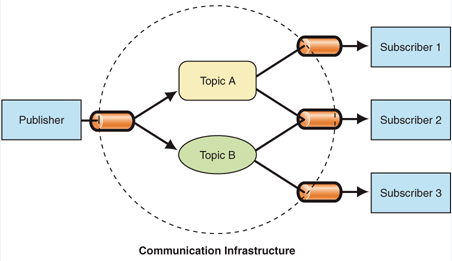
\includegraphics[width=0.6\textwidth]{pub_sub.PNG}
	\caption{Publish/Subscribe design pattern}
	\label{figure:pubsub}
\end{figure}

\subsection{Onboard nodes}


The most relevant apps that are started at boot can be divided in groups. \\

\noindent
\paragraph{System applications} Those kind of nodes manage the internal and external process communications , logging and testing. They provide the basic services on which the other modules rely:	
\begin{itemize}
	\item mavlink - is dedicated to pack and unpack mavlink messages.
	\item sdlog2 - takes relevant topics and creates a log file on sd card at every flight.
	\item test - mainly used for troubleshooting.
	\item uOrb - inter-process communication middleware .
\end{itemize}
\paragraph{Drivers} As one may imagine, those nodes represent the layer between hardware and software. They manage the communication with sensors, ports and buses:
\begin{itemize}
	\item esc\_calib - calibration of the electronic speed controllers for motors.
	\item fmu - manages the board input and output pins.
	\item GPS - GPS reciever driver
	\item pwm - command the pwm to be sent to motor controllers
	\item sensor - communication with various sensors (inertial, baro)
\end{itemize}
\paragraph{Attitude and position estimators} Those modules are responsible for position and attitude estimation, they are part of the core of the flight stack:
\begin{itemize}
	\item position\_estimator\_inav - estimates position with inertial sensor, gps and mocap measuraments.
	\item att\_estimator\_ekf - estimates attitude using inertial sensors.
\end{itemize}
\paragraph{Multirotor Attitude and Position Controllers} Those are the key modules regarding this thesis. They implements the algorithms for position and attitude control:
\begin{itemize}
	\item mc\_pos\_control - position controller
	\item mc\_att\_control - attitude controller
\end{itemize}

\paragraph{Flight safety and navigation} Those are the key modules regarding this thesis. They implements the algorithms for position and attitude control:
\begin{itemize}
	\item commander - internal state machine which determine system states for safety (flying, idle , emergency , on ground)
	\item navigator - highest level of abstraction, it implements mission following and failsafe
\end{itemize}

\subsection{State machine overview}

The system relies on a state machine in order to manage what it can and cannot do at a particular moment. The main task of this module is to assure safety from an high level point of view. Other safety procedures are implemented also on a lower level on hardware. \\

\noindent
The main states are \textit{ARMED , STAND-BY , INIT , ERROR} and \textit{UNLOCKED}. At the moment the user turns on the robot, the state machine is in \textit{INIT} state. Here all the procedure for sensor initialization and checklists are done. The next state then becomes \textit{STAND-BY} where IRIS waits for orders. By manually pressing a safety button, the state changes to UNLOCKED and back to STAND-BY by pressing again the button. In UNLOCKED state, the motor are electrically connected to the power source thus they can be armed. With a button on the remote control, the motors are armed and start spinning with idle velocity and the robot can fly. From any state, an error signal may arrive changing the actual configuration to ERROR. Here the motors are turned off after the automatic landing procedure and the robot must be rebooted. Those concept are depicted in figure \ref{figure:iris_state}.

\begin{figure}[h]
	\centering
	\noindent
	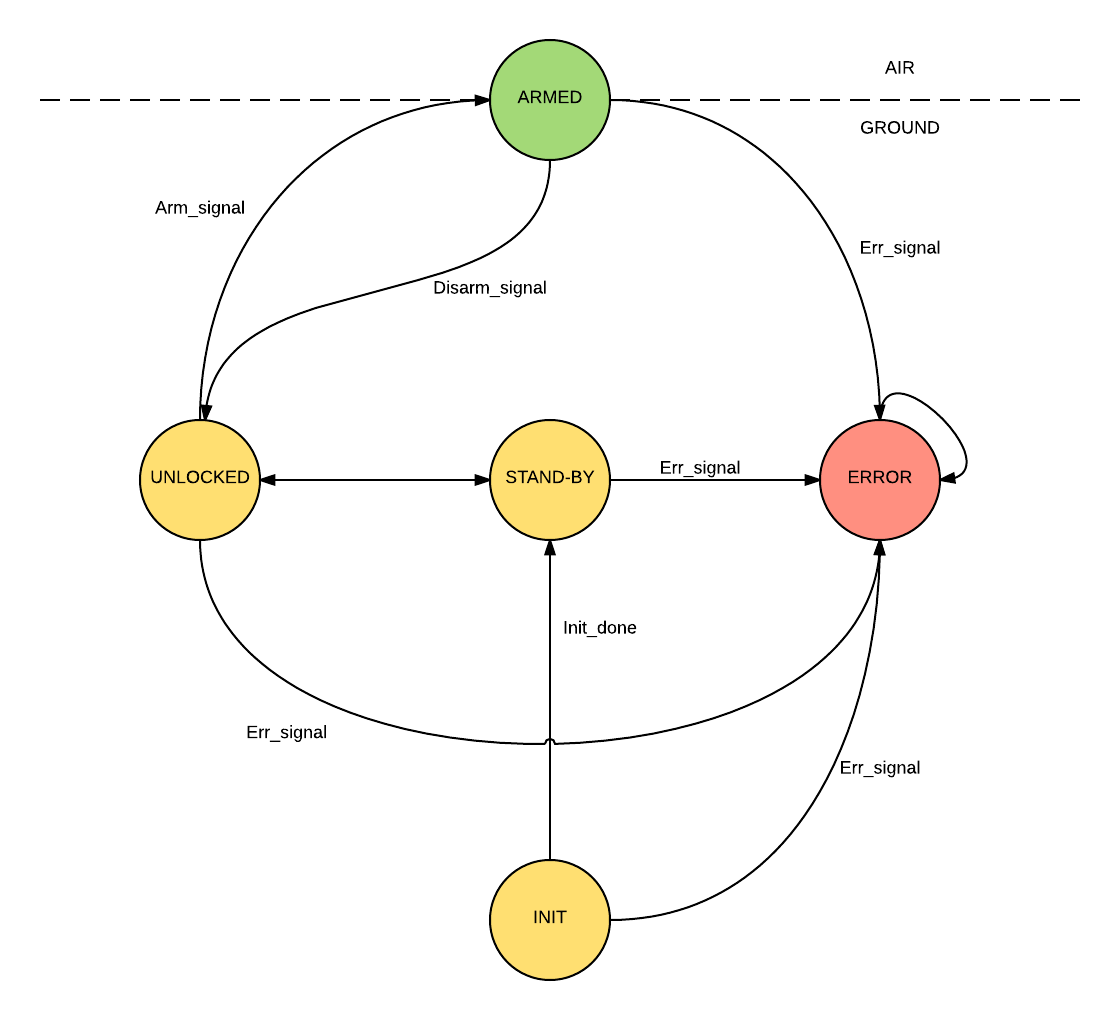
\includegraphics[width=0.7\textwidth]{iris_state.png}
	\caption{IRIS state machine}
	\label{figure:iris_state}
\end{figure}


\section{Estimation modules}

Since I am using an older version of PX4 because it is stable and well tested, the estimation occurs in two different modules. The first module, called \textit{position\_estimator\_inav} , is used to estimate the position of the quadcopter while the second, named\textit{ att\_estimator\_ekf }, estimates the attitude. The choice of dividing in two different processes the estimation phase  is mainly because attitude has an higher dynamics than position, this gives the possibility to run the attitude estimator at a frequency higher than the position estimator thus having better results.

\subsection{Position estimator}

The position estimator is based on inertial model and optimized for multirotors. It reads multiple sensors and estimates 3D position and velocity, in local and global frames. It is a fixed gain estimator and it relies on the following sources with the respective gains:
\begin{table}[H]
		\centering
	\begin{tabular}{l l r}
		\textbf{Sensor} & \textbf{ID} & \textbf{Gain} \\ \hline
		Accelerometer (for altitude) & Used as an absolute measure & - \\
		Barometer (gives absolute altitude)  & INAV\_W\_Z\_BARO & 0.0001  \\
		Accelerometer (for x and y) & Used as an absolute measure & - \\
		GPS altitude & INAV\_W\_Z\_GPS\_P & 0.005 \\
		GPS Position & INAV\_W\_XY\_GPS\_P & 1 \\
		GPS Velocity & INAV\_W\_XY\_GPS\_V & 2 \\
	    GPS climb rate & INAV\_W\_Z\_GPS\_V & 2 \\	
		Mocap estimate ( altitude ) & INAV\_W\_Z\_VIS\_P & 5 \\
		Mocap estimate ( altitude ) & INAV\_W\_XY\_VIS\_P & 7 \\
	\end{tabular}
	\caption{Correction gains and available measures}
	\label{tab:corrgain}
\end{table}
\noindent
\textbf{Note}: the accelerometers are used as an absolute measure, thus treated as the input of the system used for prediction (equation \ref{eq:prediction}). Moreover I changed the gain \textit{INAV\_W\_Z\_BARO} from 50 to 0.0001 because the sensor gives the absolute altitude above sea level while the mocap gives the height respect to the earth frame (the floor of the room). This causes a mismatch in the two measures leading to false prediction with a constant offset, hence the gain for the barometer is set very low.

\subsubsection*{Working principle of position estimator}
The algorithm for position estimation is divided in two phases: prediction and update. The model used for \textbf{prediction} is the following: 

\begin{equation}
	\begin{aligned}
	\boldsymbol{x_k}(\boldsymbol{x_{k-1}}, dt , \boldsymbol{a})& = \boldsymbol{x_{k-1}} + \boldsymbol{v_k}dt + \frac{1}{2}\boldsymbol{a}) dt^2 \\
	 \boldsymbol{v_k} ( \boldsymbol{v_{k-1}} ,\boldsymbol{a} , dt)& = \boldsymbol{v_{k-1}} + \boldsymbol{a}dt
	\end{aligned}
	\label{eq:prediction}
\end{equation}
where the vector $\boldsymbol{x_k}$ encodes the position in earth frame, the vector $a$ represent the acceleration in each axis given by the accelerometer, $v_k$ is the vector of velocities and $dt$ is the time different between the steo $k$ and $k-1$.\\

\noindent
In compact form the we can write the system as the following:
\begin{equation}
	\begin{aligned}
	\boldsymbol{F_k}(\boldsymbol{x_{k-1}}, dt ,\boldsymbol{v_{k-1}}, \boldsymbol{a})& = \begin{bmatrix}\boldsymbol{x_k}\\\boldsymbol{v_k}\end{bmatrix}\\
	\boldsymbol{y_k}& = H \boldsymbol{F_k}
	\end{aligned}
	\label{eq:predictioncompact}
	\end{equation}
where $\boldsymbol{y_k}$ is the output  (from sensors) and the H matrix relates the state with the measurements. \\

\noindent
Equation \ref{eq:predictioncompact} is usually called \textbf{prediction}. It means that with the last available estimate of  $[\boldsymbol{x_{k-1}},\boldsymbol{v_{k-1}}]$ and the actual value of the acceleration $\boldsymbol{a}$ (input of the model) given by the accelerometers, we can predict what could be the next value for $\boldsymbol{F_k}$ and by consequence the output vector $\boldsymbol{y_k}$. \\

\noindent
The last item is the \textbf{correction} or the calculation of the actual estimated value for the state. The correction equation takes the following form:
\begin{equation}
	\boldsymbol{F_k^{est}} = \boldsymbol{F_k^p}(\boldsymbol{x_{k-1}}, dt ,\boldsymbol{v_{k-1}}, \boldsymbol{a}) + L(\boldsymbol{y_k} - \boldsymbol{y_k^p})
	\label{eq:observer}
\end{equation}
meaning that the estimated (corrected) state $\boldsymbol{F_k^{est}}$ is equal to the \textbf{prediction} calculated in equation \ref{eq:predictioncompact} (the superscript p stands for prediction) plus the \textbf{innovation} $L(\boldsymbol{y_k} - \boldsymbol{y_k^p})$. The innovation term is composed by $L$ which is a diagonal matrix with the values of the correction gains listed in table \ref{tab:corrgain} for each sensor and the difference of the \textbf{actual measure read by the sensor}, namely $\boldsymbol{y_k}$, with the predicted output $\boldsymbol{y_k^p}$ calculated in \ref{eq:predictioncompact}. \\

\noindent
At the end the results are  published on \textit{vehicle\_local\_position} topic.

\subsection{Attitude estimator}

Attitude estimation is a bit more complex being a faster dynamics and accurate results are needed. This module relies on an extended Kalman filter, which is the non linear version of the very famous linear quadratic estimator. The model is of the form:
\begin{equation}
	\begin{aligned}
	\boldsymbol{x_{k+1}}& = \boldsymbol{f(\boldsymbol{x_k}, \boldsymbol{u_k})} + \boldsymbol{\xi_k} \\
	\boldsymbol{y_k}& = \boldsymbol{ g(\boldsymbol{x_k}) } + \boldsymbol{\eta_k}
	\end{aligned}
\end{equation}
where $[\boldsymbol{\xi_k} \sim N(0,Q), \boldsymbol{\eta_k} \sim N(0,R) ]$ are gaussian noises on the system and on the measurements with zero mean and [Q,R] covariances. The available sensors used are: \begin{itemize}
	\item magnetometer - for calculating magnetic field on the three robot axis (in robot frame).
	\item gyroscope - for the calculation of angular rates in body frame (p,q,r).
	\item accelerometer - for retrieving the value of the acceleration (e.g estimation of the vertical through gravity).
	\end{itemize}

\noindent
The model used is the rotational part of the system \ref{eq:mathfullmodel} (last six equations) with the angular accelerations plus the three value of the magnetic field given by the magnetometer. A well detailed description of the algorithm for this particular case is given in \cite{attekf}.

\noindent
\paragraph{Yaw estimation} The lab environment presented a couple of issues regarding the measure of the magnetic field. Being indoor, with electronic equipments and with electrical cables passing under the floor, the magnetic field is not constant along the room volume. This causes bad estimates for the yaw given by the magnetometer. Being yaw dynamics pretty slow with respect to roll and pitch, we can estimate it off board with a simple trick.\\

\noindent
Let $\boldsymbol{mag}^B = \begin{bmatrix}mag_x\\mag_y\\mag_z\end{bmatrix}$ the magnetic field vector in body frame given by the magnetometer and fed to the attitude estimator. Since the earth magnetic field is inclined by almost 30 degrees downwards and pointing north, we can fake it and decide ourself where the north is. Hence let $\boldsymbol{mag^E}$ = $\begin{bmatrix}1\\0\\0.4\end{bmatrix}$ meaning that $x^E$ becomes the north. The attitude estimator accept the magnetometer output in body frame hence the "fake" value we provide, by hacking in the module source file, becomes:
\begin{equation}
	 \boldsymbol{mag^B} = {}^BR_E \boldsymbol{mag^E}
\end{equation}
where  ${}^BR_E$ is the transpose of $R$ which depends on attitude angles. Roll and Pitch are estimated on board but the yaw is obtained by the mocap measure, thus we can construct the rotation matrix and calculate the rotate magnetic field in body frame. This approach works, is simple and gives us the possibility to choose where the north( yaw = 0) is without having the problem of alignment of $x^E$ with the North-South line.

\section{Controller architecture}

As stated in chapter \ref{chap:second}, those modules implement PIDs controller. The architecture is in the form of what is called a cascaded structure, a very common practice in control design for flying vehicles. 

The basic idea is to break up the dynamics of the quadrotor and face the problem piece by piece \cite{Mellinger2012}. Thus, the design is divided in four sub controllers placed in a cascaded fashion one after the other. Each controller generates the input for the next one and takes the output of the previous. From the highest to the lowest level we have:\textit{ position control}, \textit{velocity control}, \textit{attitude control} and\textit{ motor control}. In the purpose of this thesis, dynamics of motor control are not analyzed but just a brief overview is given. 

The \textbf{position controller} calculates the velocities set points in the three directions which are fed to the velocity controller. The task of the \textbf{velocity controller} is to track those set points by generating attitude reference signals and total thrust. The desired angular pose is tracked by the \textbf{attitude controller} which generates the desired torques as input of the \textbf{mixer}. The role of the mixer is to calculate each rotor angular speed in order to track the desired signal. This is simply done by inverting equation \ref{eq:inputmixmatrix} and expressing the angular speed vector in function of the input vector $U$ obtaining:\begin{equation}
H^{-1}\begin{bmatrix}
T^B\\\tau_\phi\\\tau_\theta\\\tau_\psi
\end{bmatrix} = \begin{bmatrix}
\omega_1^2\\\omega_2^2\\\omega_3^2\\\omega_4^2
\end{bmatrix}
\end{equation}
where the left hand side vector is the output of the attitude (for torques) and position (for thrust) controllers while the right hand side vector is the square of the desired rotor angular speeds. The matrix $H$ is the mixer matrix, it is specific for the robot configurations and it is usually given as a parameter file from the quadcopter designer. At the end of the chain there is the motor controller which, through PWM, assures the convergence to the desired spinning velocity. 

Note that those controllers run at different rates, from the position controller which has the lowest rate to the attitude controller which have the highest. Moreover the following assumption is made: \textbf{in the chain, one controller converges faster than its previous one}. This is necessary otherwise the cascade will not work properly. Those concepts are represented in figure \ref{figure:controlarch}.

\begin{figure}[h]
	\centering
	\noindent
	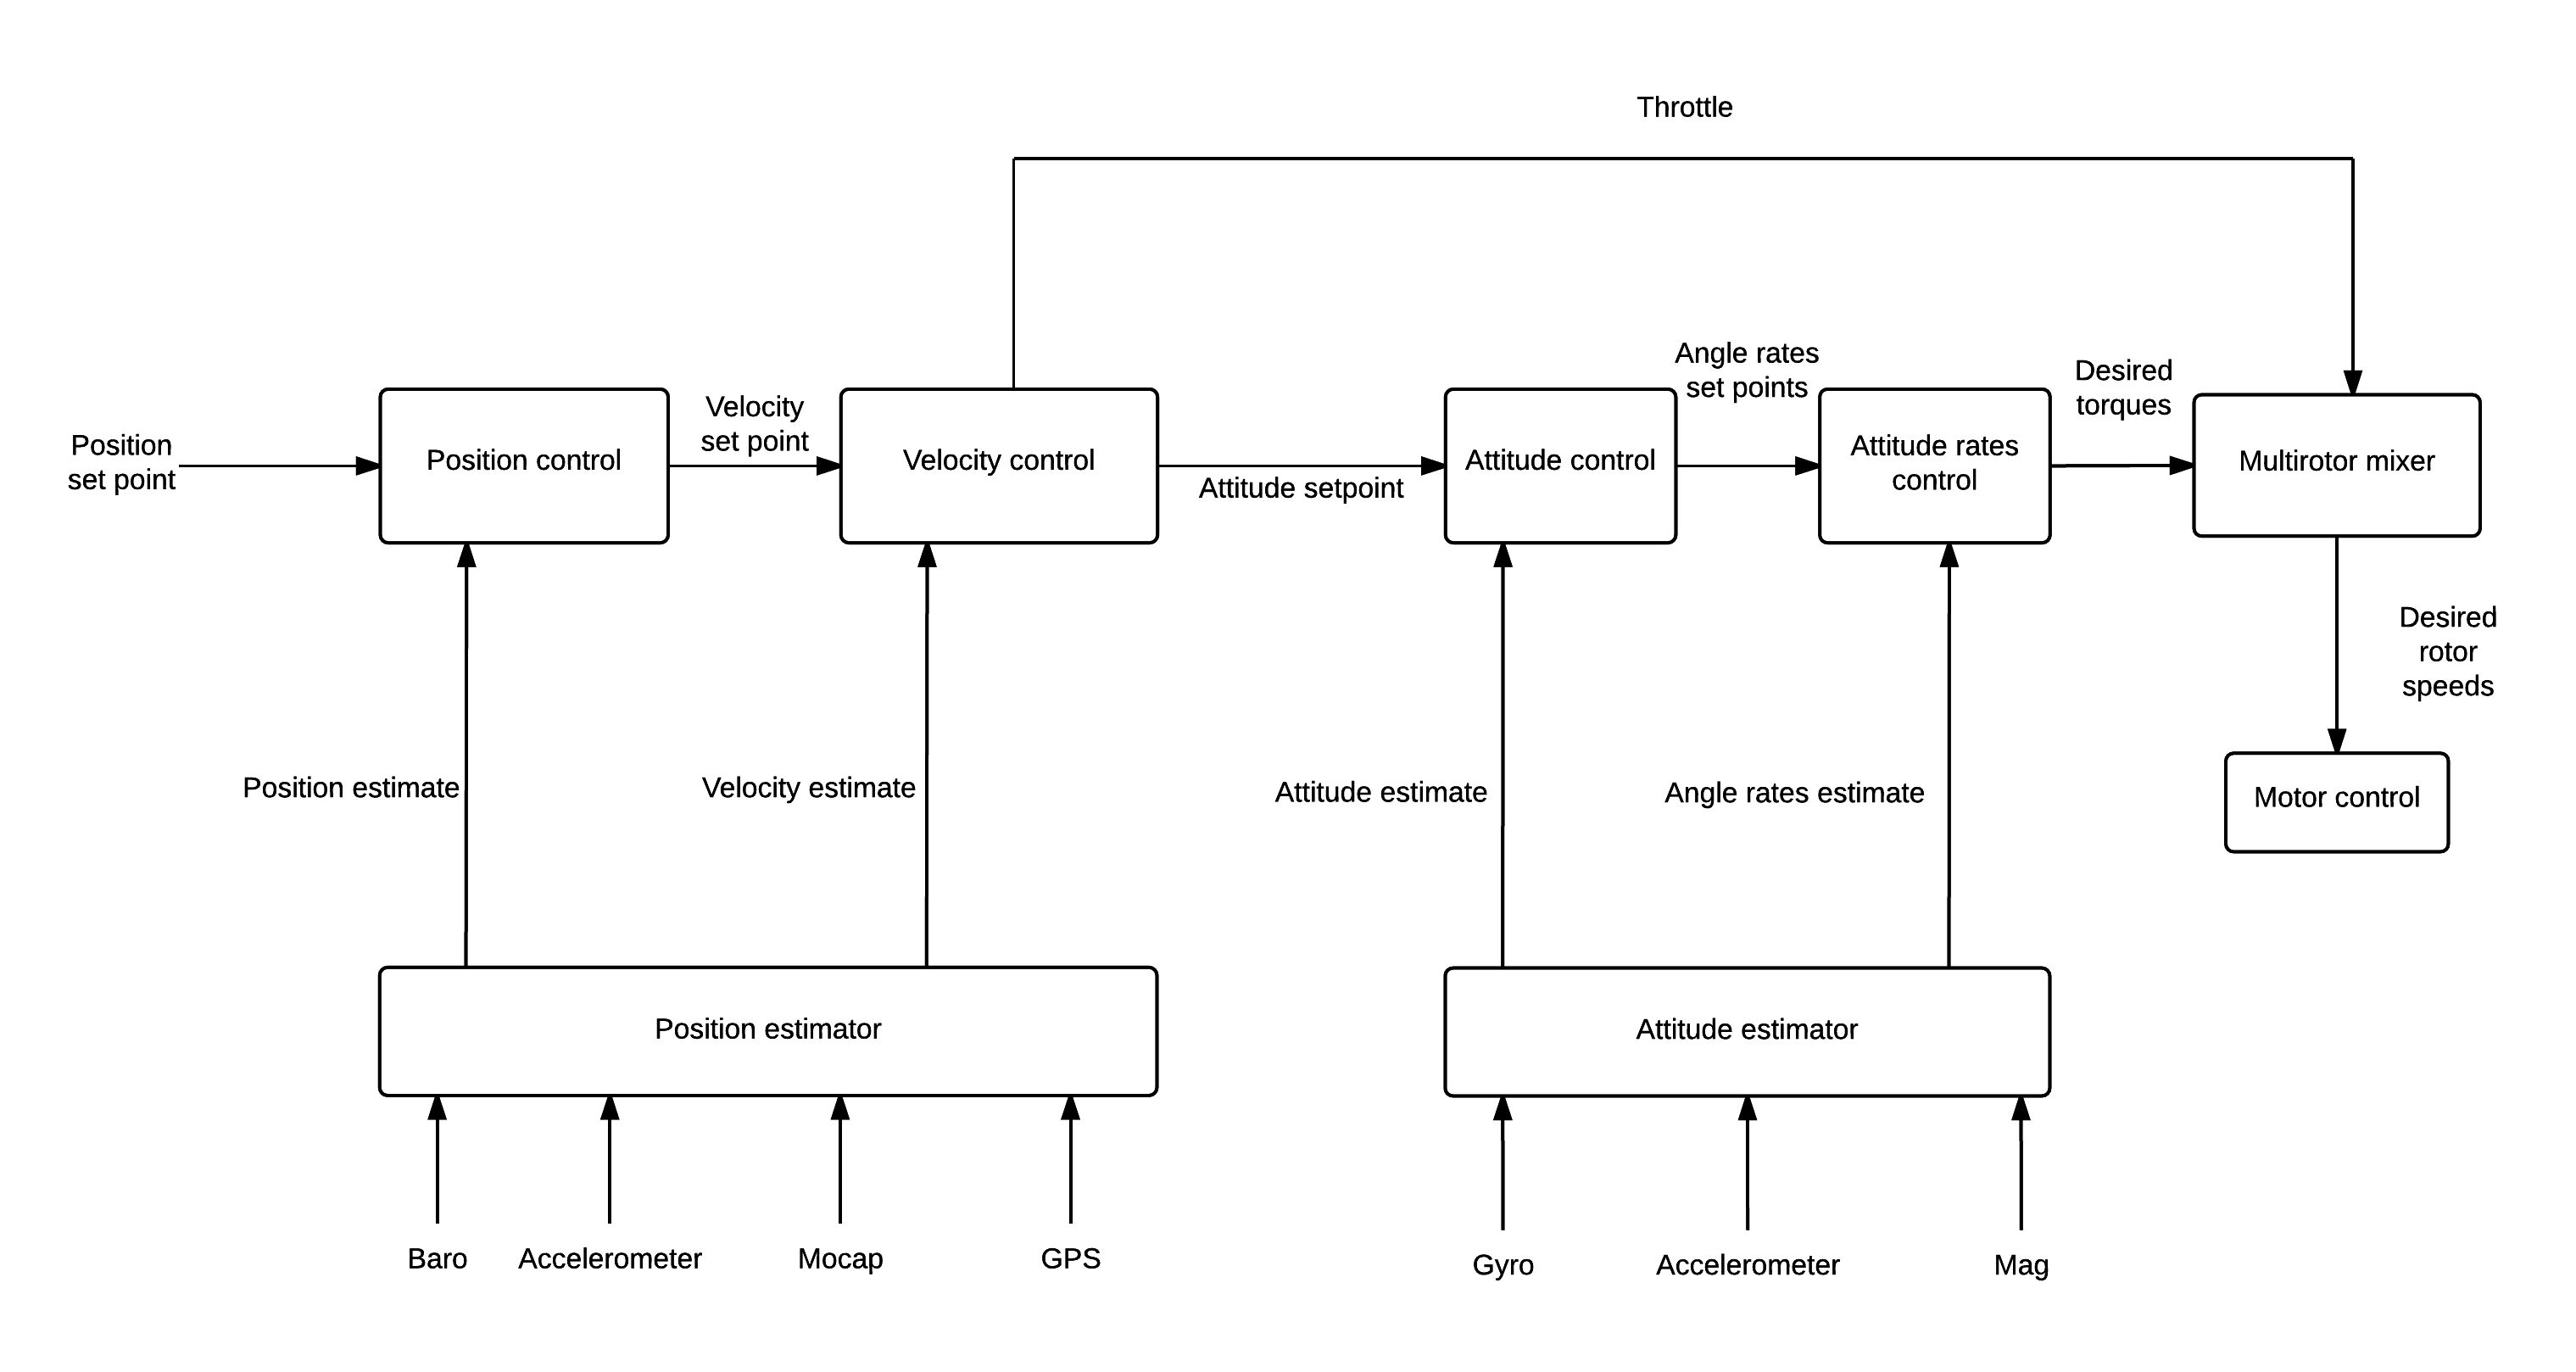
\includegraphics[width=1\textwidth]{control_arch.png}
	\caption{Controller overall structure}
	\label{figure:controlarch}
\end{figure}

\noindent
For the IRIS, three main modes are available: \begin{itemize}
	\item manual - the signals from the radio command are fed directly into the mixer
	\item altitude stabilized - throttle signal is calculated by the controller in order to track an altitude set point given by the user with the radio command. Attitude is still manual.
	\item position stabilized - the full position set point, \textbf{given by the software architecture}, is tracked by the controller chain.
\end{itemize}
\noindent
\textbf{Note:} in position stabilized usually the  set point is given by the radio command, I changed the autopilot in order to bypass the radio and send set points with the software architecture. Altitude stabilized is used for emergency since one can easily switch mode with a button on the radio.


\subsection{Position controller}
The position control is straightforward. First the position error is calculated with the feedback from the inertial estimator \begin{equation}
	\boldsymbol{e_p} =\boldsymbol{pos_{sp}} - \boldsymbol{pos}
\end{equation}
and then the desired velocity vector is generated with a proportional control law having:
\begin{equation}
	\boldsymbol{vel_{sp}} = K_p \boldsymbol{e_p}
\end{equation}
where $K_p = 1$ is the proportional gain. $\boldsymbol{pos}$, $\boldsymbol{pos_{sp}}$ and $\boldsymbol{v_{sp}}$ are 3-elements vectors and they represent respectively the actual robot position in earth frame, the position target set by the software architecture and the generated velocity setpoint.

\subsection{Velocity controller}
Velocity control occurs in two stages. First a desired thrust vector is calculated with a PID control law and then the desired attitude is generated from the thrust vector. The velocity error is defined as:
\begin{equation}
 \boldsymbol{e_v} =  \boldsymbol{vel_{sp}} - \boldsymbol{vel}
\end{equation}
and the desired thrust vector in earth frame
\begin{equation}
 \boldsymbol{th_{sp}} = K_p^{vel}  \boldsymbol{e_v} + K_d^{vel}  \boldsymbol{\dot{e}_v} + K_i^{vel} \int  \boldsymbol{e_v}
\end{equation}
with $ [K_p^{vel} ,  K_d^{vel} ,  K_i^{vel}] = [0,0,0]$  and gains are diagonal matrices with the values for x y and z in order to be able to set different gains for different dynamics. At this point we can calculate attitude set points, in the form of rotation matrix to avoid singularities, from thrust vector. The desired z axis of the robot is
\begin{equation}
	\boldsymbol{z^B_{des}} = - \frac{\boldsymbol{th_{sp}}}{\lVert\boldsymbol{th_{sp}}\rVert} 
\end{equation}
since the thrust vector points up and z down. Next, from the yaw value $\psi$ given by the attitude estimator, we calculate the intermediate vector for axis y in XY plane
\begin{equation}
	\boldsymbol{y_c} = [-sin(\psi) , cos(\psi),0]^T
\end{equation}
and then with the cross product the desired robot x axis is calculated
\begin{equation}
	\boldsymbol{x^B_{des}} = \boldsymbol{y_c} \times \boldsymbol{z^B_{des}}
\end{equation}
As consequence the desired robot y axis is
\begin{equation}
\vspace{2ex}
\boldsymbol{y^B_{des}} = \boldsymbol{z^B_{des}} \times \boldsymbol{x^B_{des}}
\end{equation}
\noindent
The desired rotation matrix, ready to be sent to the attitude controller is

\begin{equation}
\boldsymbol{R_{des}} = \begin{bmatrix}
\boldsymbol{x^B_{des}} && \boldsymbol{y^B_{des}} && \boldsymbol{z^B_{des}}
\end{bmatrix}
\end{equation}
where $[\boldsymbol{x^B_{des}} , \boldsymbol{y^B_{des}} , \boldsymbol{z^B_{des}}]$ are 3-dimensional column vectors expressed in earth frame denoting the desired axis of the body.

\noindent
Finally the total thrust $U_1$ is calculated, the first element of the input vector which is directly sent to the mixer is
\begin{equation}
	U_1 =  {\lVert\boldsymbol{th_{sp}}\rVert}
\end{equation}



\subsection{Attitude controller}

In order to calculate the last three element of the input vector $\boldsymbol{U}$, the attitude controller takes place. First thing to do is to define the rotation error between the desired rotation matrix and the actual one. Let $S = \begin{bmatrix}
0  && -c && b  \\
c  && 0  && -a \\
-b && a  && 0 
\end{bmatrix}$ be a general skew-symmetric matrix, the following is true
\begin{equation}
	S^{\wedge} = \begin{bmatrix}a\\b\\c\end{bmatrix}
\end{equation}
and the operator $\wedge$ is called vee map. Then we can define the error vector as the following:
\begin{equation}
	\boldsymbol{e_r} = \frac{1}{2} (R^T_{des} R - R^TR_{des} )^\wedge
\end{equation}
Next, similarly to the position controller, we introduce the desired angular rater in body frame as
\begin{equation}
	\boldsymbol{\Omega^B_{des}} = K_p^{rot} \boldsymbol{e_r} 
\end{equation}
and right after the angular rate error is 
\begin{equation}
	\boldsymbol{e_\omega} = \Omega^B_{des} - \Omega^B
\end{equation}
with $\Omega^B$ and $R$ given by the attitude estimator.
Finally, through PIDs controller, the command torques are generated and:

\begin{equation}
	\begin{bmatrix}
	U_2\\U_3\\U_4
	\end{bmatrix} =  K_p^{\omega}  \boldsymbol{e_\omega} + K_d^{\omega} { \boldsymbol{\dot{e}_\omega}} + K_i^{\omega} \int \boldsymbol{e_\omega}
\end{equation}
where the gains are diagonal matrices with the value of the gain of eac dynamics (roll, pitch and yaw rates).


\section{Results and validation}









